\documentclass[10pt,a4paper]{article}
\usepackage[utf8]{inputenc}
\usepackage[T1]{fontenc}
\usepackage[polish]{babel}
\usepackage{hhline}
\usepackage{pgfplots}

\usepackage{multicol}
%\usepackage{slashbox}
\usepackage{graphicx}
\usepackage{caption}
\usepackage{subcaption}
\usepackage{colortbl}

\usepackage{geometry}
\geometry{a4paper, total={170mm,257mm}, left=20mm, top=20mm }

\author{Jan Techner 132332 i Sebastian Maciejewski 132275 \\ grupa I1}
\title{Analiza zdjęć - rozpoznawanie par symboli na kartach Dobble}
\date{18 listopada 2018}
\setlength{\parindent}{0pt}
\newcommand{\forceindent}{\leavevmode{\parindent=3em\indent}}

\begin{document}
\maketitle
\section{Wstęp}

\forceindent Program, który napisaliśmy ma za zadanie pobrać od użytkownika zdjęcie stanu rozgrywki (od 2 do 5 graczy) i zaznaczenie na tym zdjęciu identycznych symboli występujących na różnych kartach. \\
Nasz algorytm rozpoczyna pracę od podziału zdjęcia na pojedyncze karty, dodania dla każdej karty listy rozpoznanych na niej symboli, a następnie umieszczenia karty w 
liście wyciętych kart. Ten fragment programu jest kluczowy dla końcowego rezultatu, bowiem to od jakości rozpoznania kart i symboli zależy skuteczność ich porównywania. \\

W skrócie: proces wycinania polega na znalezieniu krawędzi po zastosowaniu filtru threshold dla zdjęć z ciemnym tłem lub specjalnego filtru threshold po 3 kanałach R, G, B (który to filtr pozwala uzyskać wyjątkowo dokładne obrysy, ponieważ analizuje każdy kanał z osobna, następnie złączając je w jeden obraz) dla zdjęć z jasnym (białym) tłem. W przypadku ciemnego tła symbole są przyporządkowywane do kart dzięki algorytmowi wykrywania konturów, który zwraca drzewiastą sktrukturę. Na jej podstawie można rozpoznać czy symbol zawiera się w karcie. Ponowne zastosowanie filtru threshold, tym razem w wersji RGB na jednej wyciętej karcie, umożiwia dokładne rozpoznawanie symboli po powtórnym wywołaniu algorytmu wyszukiwania konturów. W przypadku zdjęć z jasnym tłem algorytm wykrywania konturów zwraca same symbole, które następnie są grupowane w karty na podstawie ich wzajemnych odległości na zdjęciu - w ten sposób mamy możliwość wykrycia kart mimo niekontrastowego tła zdjęcia. Tak rozpoznane symbole są zapisywane jako małe wycinki zdjęcia (najmniejsze prostokąty, w których mieści się symbol) w tablicy symboli dla danej karty. \\

Kiedy już uda się wyciąć karty i symbole, przychodzi czas na porównywanie ich ze sobą - w tym celu dla każdej pary kart (co można, nie zmniejszając ogólności rozumowania, sprowadzić do przypadku porównywania każdej karty poza najbliższą środkowi zdjęcia z tą najbardziej środkową kartą) wywoływana jest funkcja porównująca, której zadaniem jest zaznaczenie na oryginalnym zdjęciu pary symboli, które odpowiadają sobie na tej parze kart. 

Działanie funkcji porównującej można rozłożyć na kilka etapów - na początek przechodzi ona po wszystkich parach symboli i oblicza różnice momentów hu, wartości kolorów (w HSV) i stosunku długości boków (najmniejszego prostokąta zawierającego cały symbol) dla każdej pary. Jeśli różnica momentów i stosunku długości jest w ustalonym przedziale akceptowalnych dopasowań, to taka para symboli jest zapisywana jako potencjalnie prawidłowe dopasowanie. Następnie dla wszystkich takich dopasowań porównywane są różnice kolorów symboli i te, których różnica kolorów jest najmniejsza są uznawane za prawidłowe dopasowanie. Między środkami tych symboli jest rysowana strzałka na głownym zdjęciu, co ma oznaczać, że te dwa symbole są identyczne z dokładnością do rozmiaru i rotacji.

\newpage

\section{Przetwarzanie - analiza przypadków}
Przyjrzyjmy się dokładniej procesowi przetwarzania w kilku przypadkach.
\subsection{Pięciu graczy, ciemne tło, naturalne oświetlenie}
Na podstawie poniższego zdjęcia oczekujemy, że program odnajdzie wszystkie 12 dopasowań z zadowalającą dokładnością:\\
\begin{center}
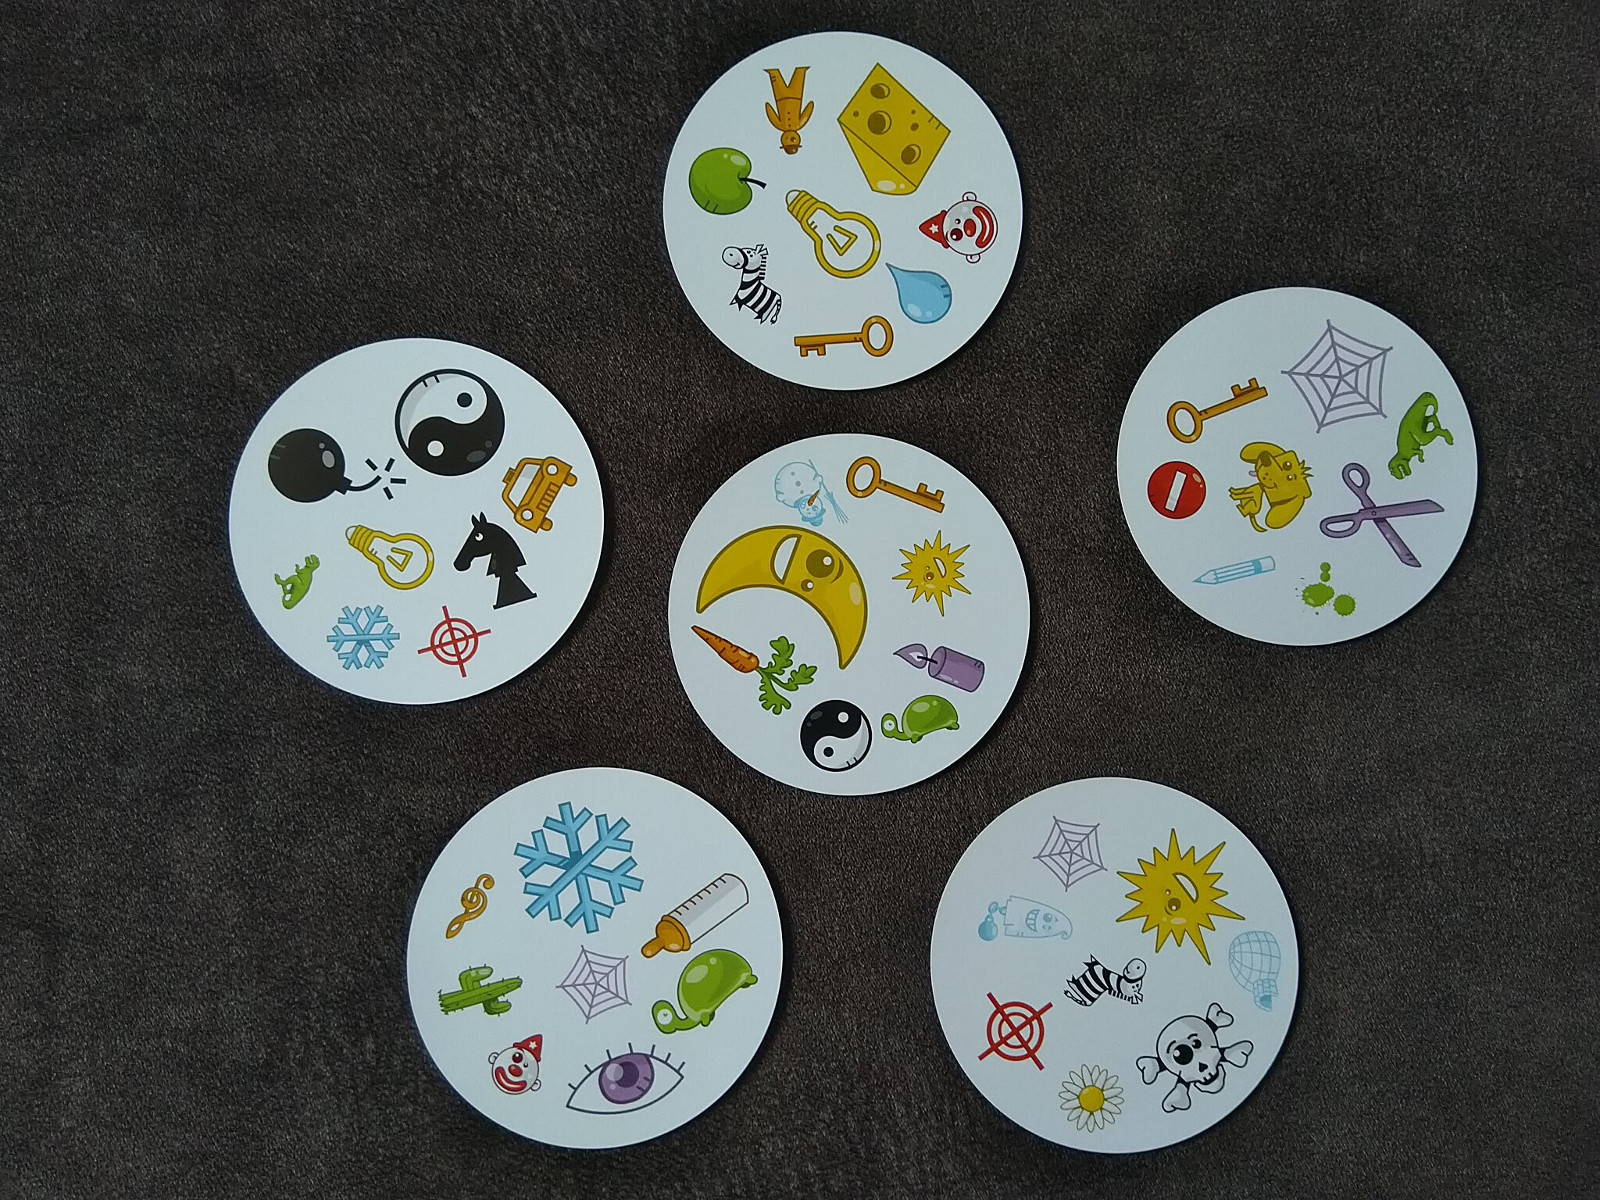
\includegraphics[scale=0.25]{2.1/dobble04.jpg}
\end{center}
Zanim wytniemy karty, musimy nałożyć odpowiednie filtry na zdjęcie, żeby móc wywołać algorytm szukający konturów. W naszym wypadku takimi filtrami są threshold, erozja i dylatacja, po których zastosowaniu zdjęcie wygląda tak:\\
\begin{center}

\includegraphics[scale=0.20]{2.1/th1.jpg}
\end{center}
Najpierw zajmujemy się wycięciem wszystkich 6 kart i wybieleniem tła (w celu prostszego użycia filtru threshold na późniejszym etapie przetwarzania). Lista wyciętych kart po tych operacjach zawiera następujące obrazy:\\
\begin{center}
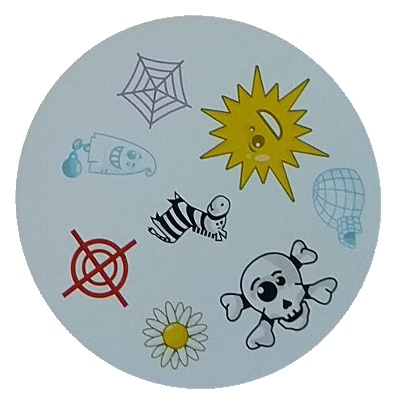
\includegraphics[scale=0.25]{2.1/card0.jpg}
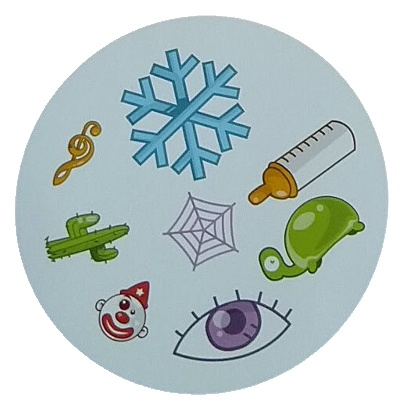
\includegraphics[scale=0.25]{2.1/card1.jpg}
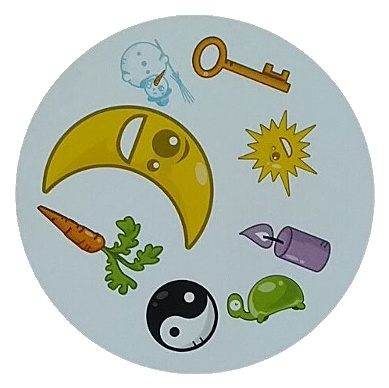
\includegraphics[scale=0.25]{2.1/card2.jpg}
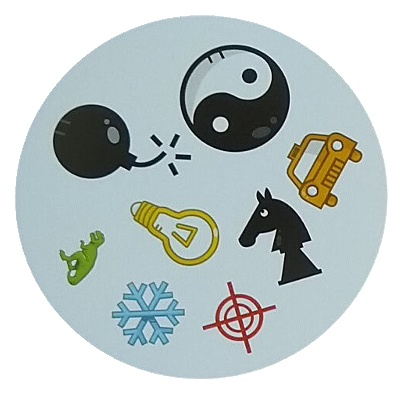
\includegraphics[scale=0.25]{2.1/card3.jpg}
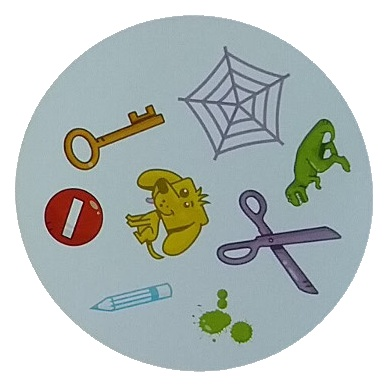
\includegraphics[scale=0.25]{2.1/card4.jpg}
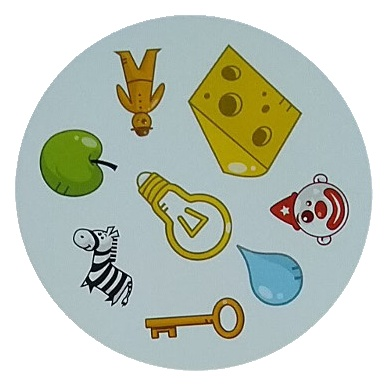
\includegraphics[scale=0.25]{2.1/card5.jpg}
\end{center}
Każda karta jest teraz indywidualnie rozjaśniana lub przyciemniana za pomocą korekcji gamma, żeby zniewlować różnice w oświetleniu wynikające np. z różnej odległości od źródła światła (w przypadku sztucznego oświetlenia).
Następnie do każdej karty stosujemy threshold RGB, żeby następnie móc odnaleźć kontury symboli. Obrazy, na których szukamy konturów wyglądają w tej chwili tak:\\
\begin{center}
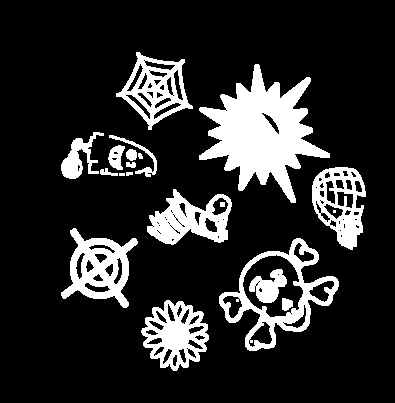
\includegraphics[scale=0.25]{2.1/0.jpg}

\includegraphics[scale=0.25]{2.1/1.jpg}
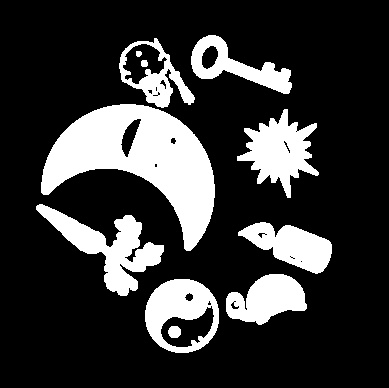
\includegraphics[scale=0.25]{2.1/2.jpg}
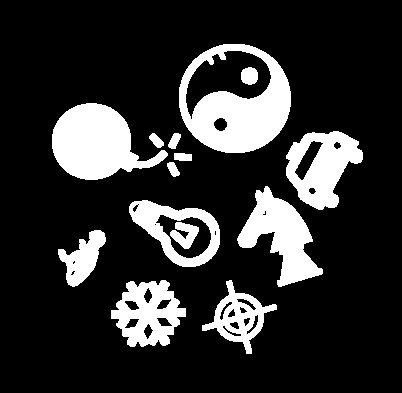
\includegraphics[scale=0.25]{2.1/3.jpg}

\includegraphics[scale=0.25]{2.1/4.jpg}
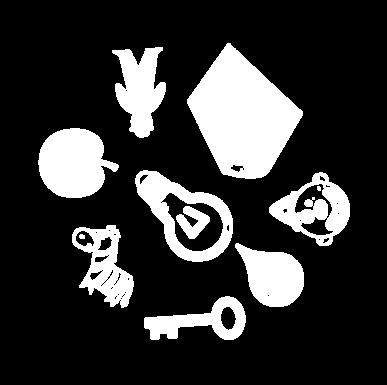
\includegraphics[scale=0.25]{2.1/5.jpg}
\end{center}
Po odnalezieniu konturów każdego symbolu i wycięciu najmniejszego prostokąta w którym się on znajduje, otrzymujemy zbiór kształtów, np. dla drugiej karty jest to:\\
\begin{center}

\includegraphics[scale=0.5]{2.1/sign10.jpg}

\includegraphics[scale=0.5]{2.1/sign11.jpg}

\includegraphics[scale=0.5]{2.1/sign12.jpg}

\includegraphics[scale=0.5]{2.1/sign13.jpg}

\includegraphics[scale=0.5]{2.1/sign14.jpg}

\includegraphics[scale=0.5]{2.1/sign15.jpg}

\includegraphics[scale=0.5]{2.1/sign16.jpg}

\includegraphics[scale=0.5]{2.1/sign17.jpg}
\end{center}
Pozostaje jeszcze usunąć (wybielić) niepotrzebne tło obrazków. Po tym etapie przetwarzania wiemy, że druga karta składa się z następujących symboli:
\begin{center}
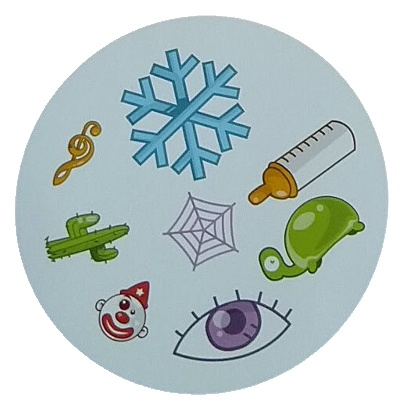
\includegraphics[scale=0.4]{2.1/card1.jpg} \\

\includegraphics[scale=0.5]{2.1/card1sign0.jpg}

\includegraphics[scale=0.5]{2.1/card1sign1.jpg}
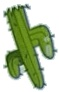
\includegraphics[scale=0.5]{2.1/card1sign2.jpg}
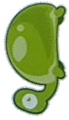
\includegraphics[scale=0.5]{2.1/card1sign3.jpg}

\includegraphics[scale=0.5]{2.1/card1sign4.jpg}

\includegraphics[scale=0.5]{2.1/card1sign5.jpg}

\includegraphics[scale=0.5]{2.1/card1sign6.jpg}

\includegraphics[scale=0.5]{2.1/card1sign7.jpg}
\end{center}
Na tym etapie pozostaje już tylko wywołanie funkcji dopasowywania dla wszystkich znalezionych kart - po jej wywołaniu otrzymujemy następujący obraz:
\begin{center}
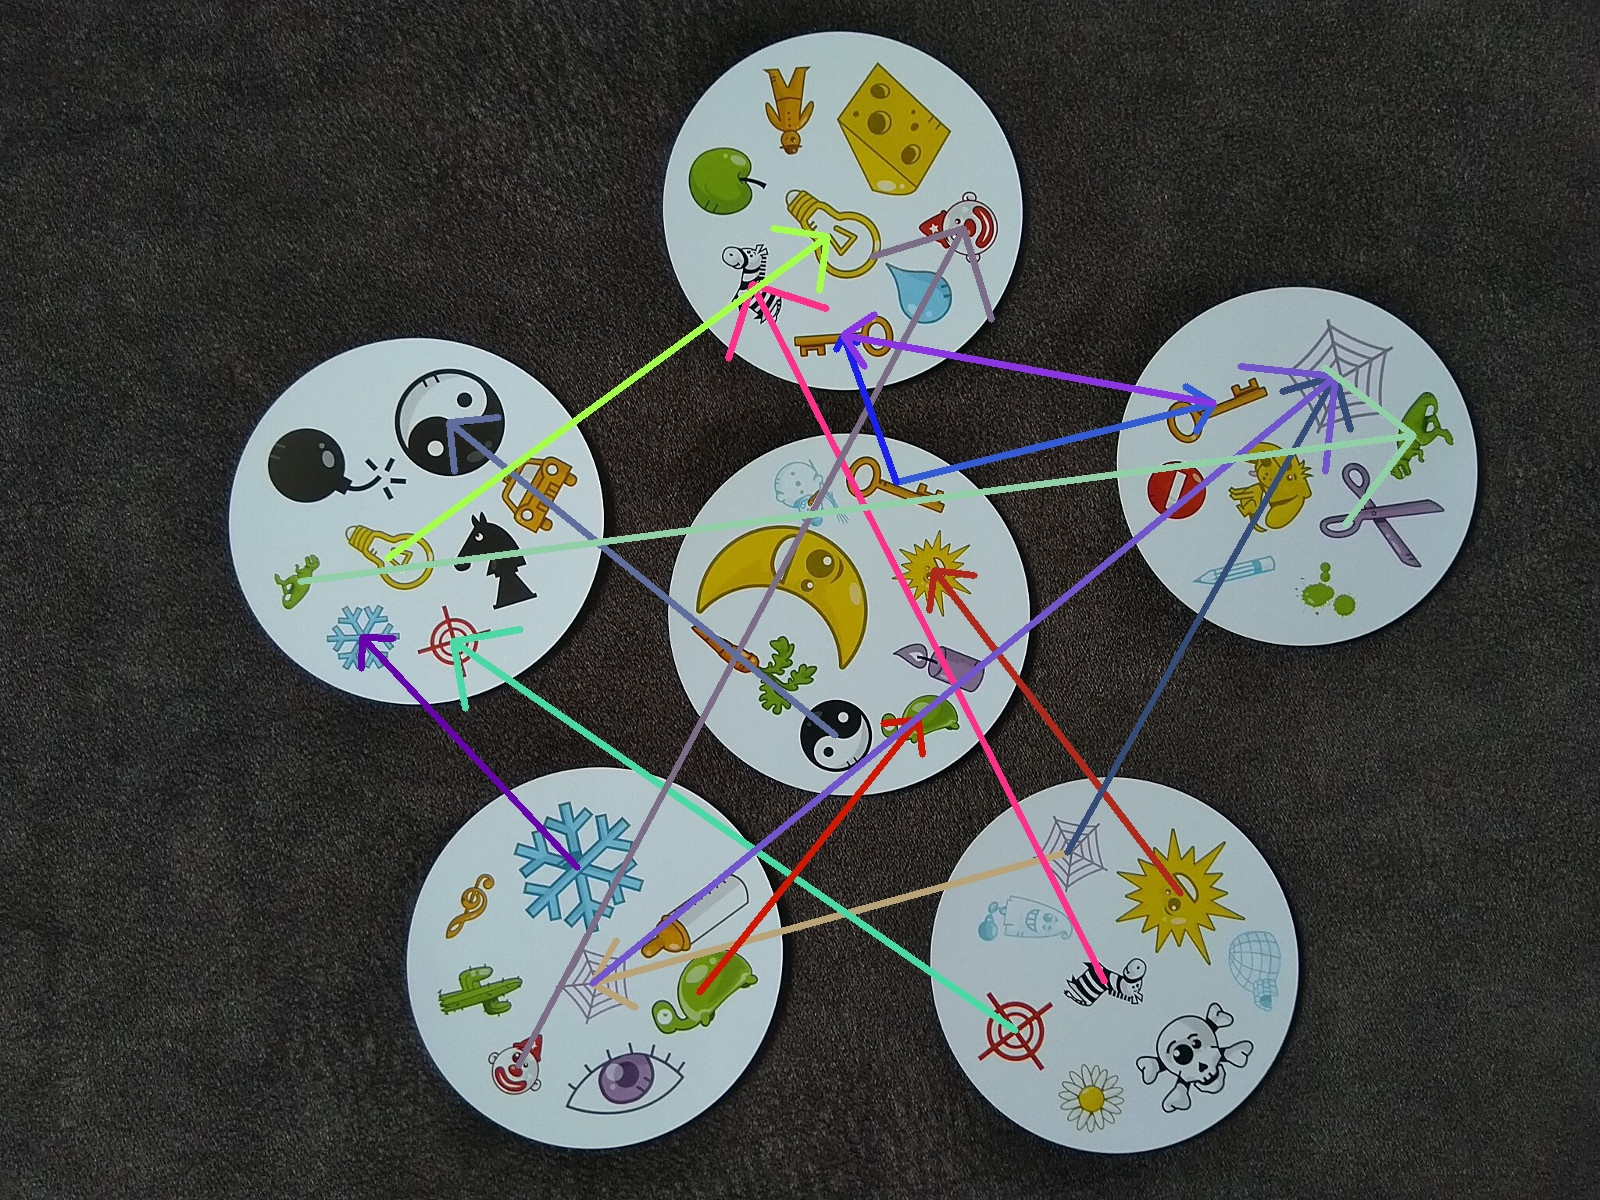
\includegraphics[scale=0.25]{2.1/img_arrows0.jpg}
\end{center}
Jak widać, w tym przypadku udało się odnaleźć 100\% dopasowań.
\newpage

\subsection{Dwóch graczy, w perspektywie, sztuczne oświetlenie, duża różnica jasności między kartami}
W wypadku tego zdjęcia liczymy na odnalezienie 3 dopasowań w trudnych warunkach oświetleniowych - lewa strona zdjęcia jest prześwietlona, dodatkowo zdjęcie jest pod kątem:\\
\begin{center}
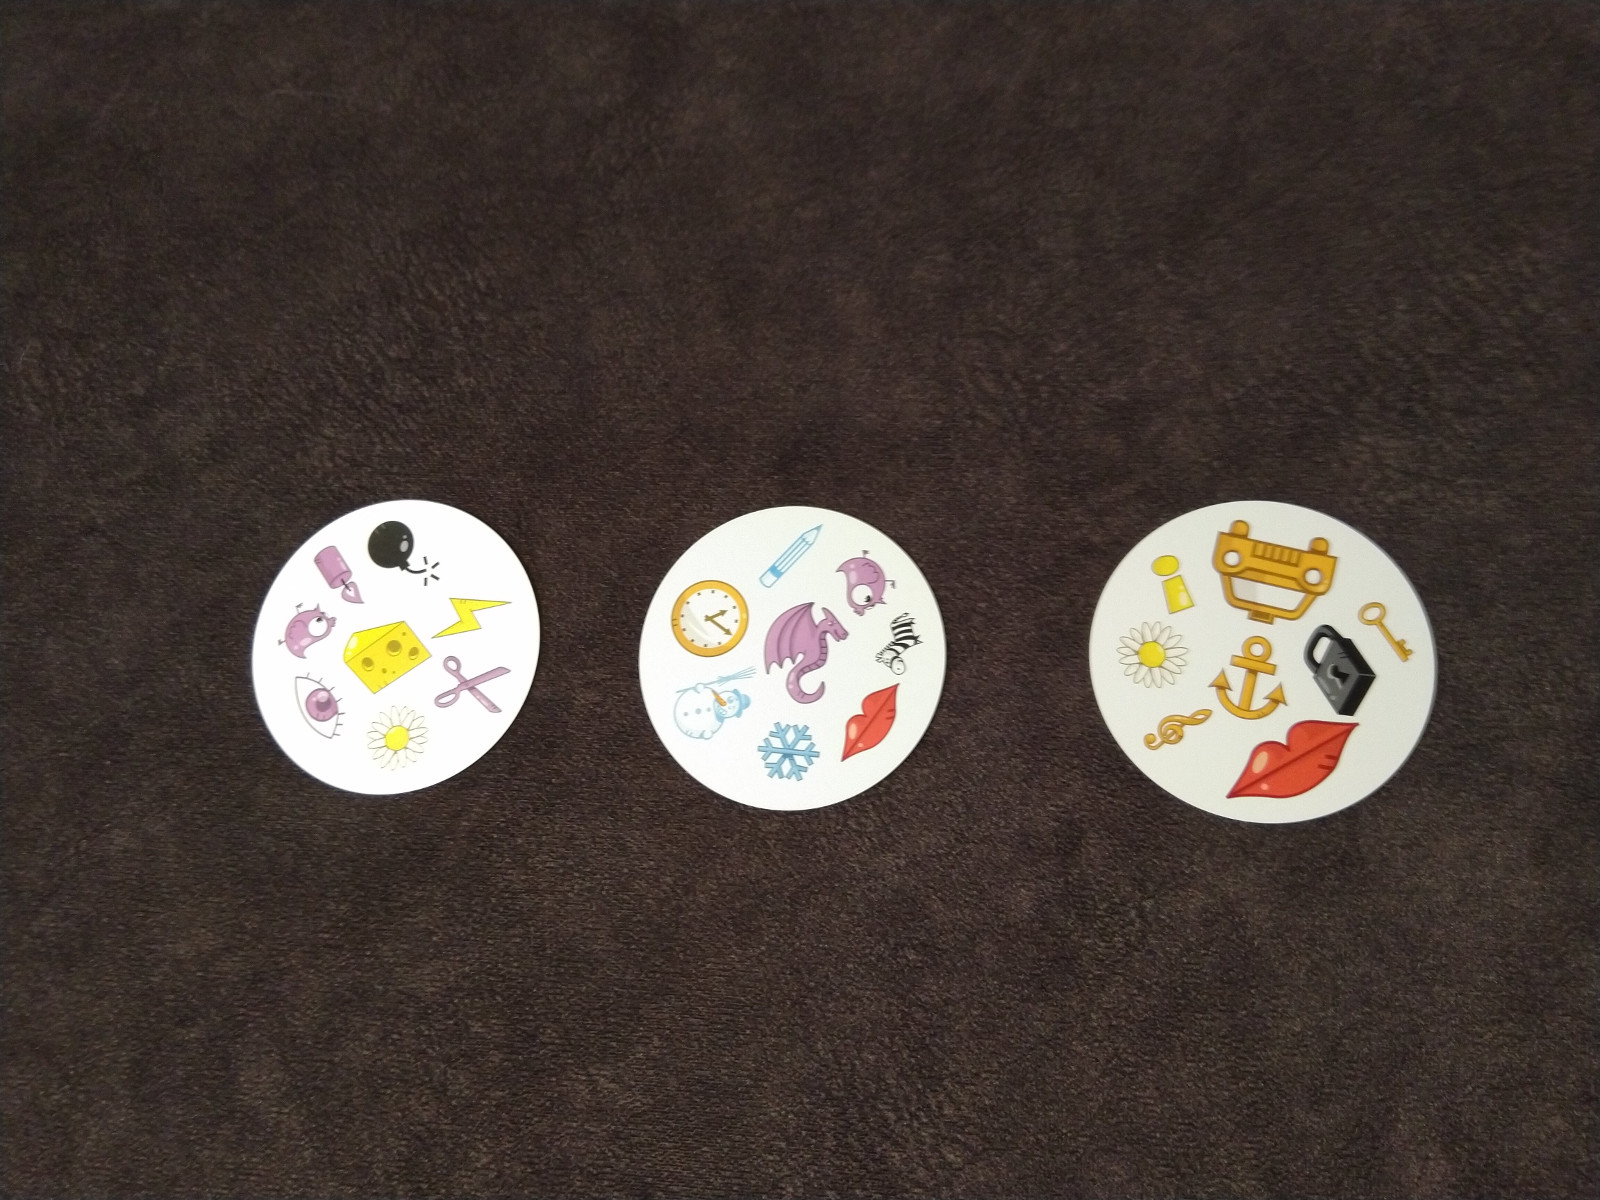
\includegraphics[scale=0.25]{2.2/dobble11.jpg}
\end{center}
Po zastosowaniu filtrów w celu wycięcia konturów dostajemy:
\begin{center}

\includegraphics[scale=0.20]{2.2/th1.jpg}
\end{center}
\newpage
Jak widać, takie filtry sprawiają że jedyne co można na tym etapie wyciąć to same karty. Po ich wycięciu postępujemy analogicznie do poprzedniego przykładu i obrazy w liście kart to:
\begin{center}
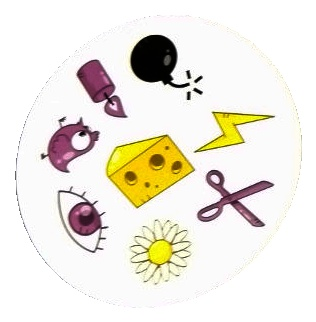
\includegraphics[scale=0.25]{2.2/card2.jpg}
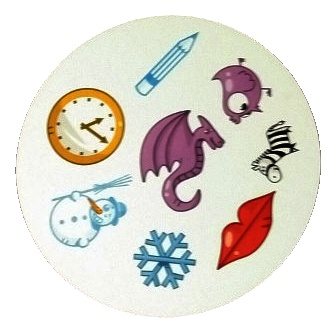
\includegraphics[scale=0.25]{2.2/card0.jpg}
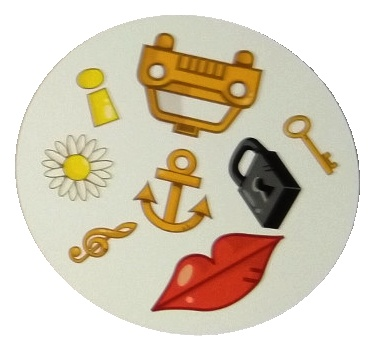
\includegraphics[scale=0.25]{2.2/card1.jpg}
\end{center}
Można tu zauważyć jak duże są różnice w oświetleniu i perspektywie poszczególnych kart na tym zdjęciu. Następnie stosujemy threshold RGB dla kart:
\begin{center}
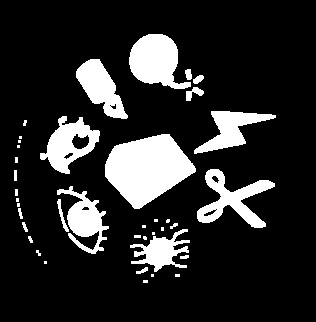
\includegraphics[scale=0.25]{2.2/2.jpg}
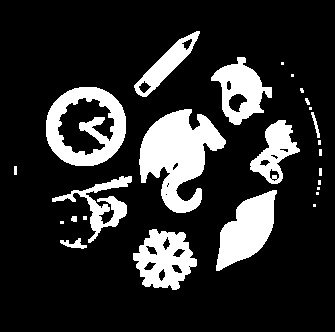
\includegraphics[scale=0.25]{2.2/0.jpg}

\includegraphics[scale=0.25]{2.2/1.jpg}
\end{center}
Po wycięciu dla danej, np. środkowej, karty kształtów dostajemy jej symbole:
\begin{center}

\includegraphics[scale=0.5]{2.2/sign00.jpg}

\includegraphics[scale=0.5]{2.2/sign01.jpg}

\includegraphics[scale=0.5]{2.2/sign02.jpg}

\includegraphics[scale=0.5]{2.2/sign03.jpg}

\includegraphics[scale=0.5]{2.2/sign04.jpg}

\includegraphics[scale=0.5]{2.2/sign05.jpg}

\includegraphics[scale=0.5]{2.2/sign06.jpg}

\includegraphics[scale=0.5]{2.2/sign07.jpg}
\end{center}
\begin{center}

\includegraphics[scale=0.5]{2.2/card0sign0.jpg}

\includegraphics[scale=0.5]{2.2/card0sign1.jpg}
\includegraphics[scale=0.5]{2.2/card0sign2.jpg}
\includegraphics[scale=0.5]{2.2/card0sign3.jpg}
\includegraphics[scale=0.5]{2.2/card0sign4.jpg}
\includegraphics[scale=0.5]{2.2/card0sign5.jpg}
\includegraphics[scale=0.5]{2.2/card0sign6.jpg}
\includegraphics[scale=0.5]{2.2/card0sign7.jpg}
\end{center}
Widać, że symbol bałwana nie wyciął się do końca z powodu bardzo dużej różnicy jasności między jednym a drugim końcem tego symbolu (dół bałwana leży blisko najmocniej oświetlonej krawędzi karty), jednak symbol wciąż zachował swoją charakterystykę kolorystyczną i większość swojego kształtu. 
\newpage
Pozostaje uruchomić algorytm porównywania:
\begin{center}
\includegraphics[scale=0.25]{2.2/img_arrows0.jpg}
\end{center}
Również w tym przypadku dokładność dopasowania to 100\% przypadków, jednak warto zauważyć jak bardzo różne pod względem koloru są symbole kwiatka na skrajnych kartach:
\begin{center}
\includegraphics[scale=1]{2.2/card1sign3.jpg}
\includegraphics[scale=1]{2.2/card2sign0.jpg}
\end{center}
Takie przypadki to jeden z powodów, dla których w naszym algorytmie porównywania kolor jest brany pod uwagę jako ostatni - przy sztucznym oświetleniu różnica w kolorach może być znacząca. W tym przypadku właśnie tak jest - środek lewego kwiatka to R: 222, G: 197, B: 17 a środek prawego to R: 249, G: 244, B: 5.
\newpage
\subsection{Czterech graczy, białe tło}
Białe tło zdjęcia to szczególnie trudny przypadek, ponieważ nie można w łatwy sposób znaleźć konturów kart. Na tym zdjęciu dodatkowym utrudnieniem jest światło, padające wyraźnie z lewej strony. Liczymy na 10 prawidłowych dopasowań.
\begin{center}
\includegraphics[scale=0.25]{2.3/dobble14.jpg}
\end{center}
Spróbujmy zastosować threshold:
\begin{center}
\includegraphics[scale=0.25]{2.3/th1.jpg}
\end{center}
\newpage
Po zastosowaniu filtru threshold widać z jakim problemem mamy tu do czynienia - karty są nieodróżnialne od tła. Spróbujmy zatem wymazać tło:
\begin{center}
\includegraphics[scale=0.25]{2.3/20.jpg}
\end{center}
Poza artefaktem w prawym dolnym rogu (ciemny róg zdjęcia) dostajemy zdjęcie, które w zasadzie jest gotowe do zastosowania wersji RGB filtru threshold w celu znalezienia symboli. Znajdujemy wszystkie symbole (łącznie z artefaktem) i wycinamy ich kontury:
\begin{center}
\includegraphics[scale=0.25]{2.3/sign02.jpg}
\includegraphics[scale=0.25]{2.3/sign03.jpg}
\includegraphics[scale=0.25]{2.3/sign04.jpg}
\includegraphics[scale=0.25]{2.3/sign05.jpg}
\includegraphics[scale=0.25]{2.3/sign06.jpg}
\includegraphics[scale=0.25]{2.3/sign07.jpg}
\includegraphics[scale=0.25]{2.3/sign11.jpg}
\includegraphics[scale=0.25]{2.3/sign12.jpg}
\includegraphics[scale=0.25]{2.3/sign13.jpg}
\includegraphics[scale=0.25]{2.3/sign14.jpg}
\includegraphics[scale=0.25]{2.3/sign15.jpg}
\includegraphics[scale=0.25]{2.3/sign16.jpg}
\includegraphics[scale=0.25]{2.3/sign17.jpg}
\includegraphics[scale=0.25]{2.3/sign20.jpg}
\includegraphics[scale=0.25]{2.3/sign21.jpg}
\includegraphics[scale=0.25]{2.3/sign22.jpg}
\includegraphics[scale=0.25]{2.3/sign23.jpg}
\includegraphics[scale=0.25]{2.3/sign24.jpg}
\includegraphics[scale=0.25]{2.3/sign25.jpg}
\includegraphics[scale=0.25]{2.3/sign26.jpg}
\includegraphics[scale=0.25]{2.3/sign30.jpg}
\includegraphics[scale=0.25]{2.3/sign31.jpg}
\includegraphics[scale=0.25]{2.3/sign32.jpg}
\includegraphics[scale=0.25]{2.3/sign33.jpg}
\includegraphics[scale=0.25]{2.3/sign34.jpg}
\includegraphics[scale=0.25]{2.3/sign35.jpg}
\includegraphics[scale=0.25]{2.3/sign36.jpg}
\includegraphics[scale=0.25]{2.3/sign37.jpg}
\includegraphics[scale=0.25]{2.3/sign38.jpg}
\includegraphics[scale=0.25]{2.3/sign39.jpg}
\includegraphics[scale=0.25]{2.3/sign40.jpg}
\includegraphics[scale=0.25]{2.3/sign41.jpg}
\includegraphics[scale=0.25]{2.3/sign42.jpg}
\includegraphics[scale=0.25]{2.3/sign43.jpg}
\includegraphics[scale=0.25]{2.3/sign44.jpg}
\includegraphics[scale=0.25]{2.3/sign45.jpg}
\includegraphics[scale=0.25]{2.3/sign46.jpg}
\end{center}
Następnie próbujemy te zarysy symboli pogrupować w karty, żeby wiedzieć w jaki sposób je porównać, oraz żeby odrzucić artefakty. Grupowanie polega na sprawdzaniu odległości między symbolami i po jego przeprowadzeniu dostajemy zbiory symboli pogrupowane w karty, np. środkowa karta to:
\begin{center}
\includegraphics[scale=0.5]{2.3/card1sign0.jpg}
\includegraphics[scale=0.5]{2.3/card1sign1.jpg}
\includegraphics[scale=0.5]{2.3/card1sign2.jpg}
\includegraphics[scale=0.5]{2.3/card1sign3.jpg}
\includegraphics[scale=0.5]{2.3/card1sign4.jpg}
\includegraphics[scale=0.5]{2.3/card1sign5.jpg}
\includegraphics[scale=0.5]{2.3/card1sign6.jpg}
\includegraphics[scale=0.5]{2.3/card1sign7.jpg}
\end{center}
\newpage
Mimo, że nie mamy zapisanych obrazów kart jako takich, to na samych zbiorach ich symboli możemy wywołać funkcję porównywania kart, bo korzysta ona ze zbioru symboli karty i współrzędnych tych symboli na zdjęciu (w celu rysowania strzałek). Po jej wywołaniu dostajemy:
\begin{center}
\includegraphics[scale=0.25]{2.3/img_arrows0.jpg}
\end{center}
Jak widać, dokładność porównania to w tym przypadku 80\%, mamy dwa błędne dopasowania - wyżej można zauważyć, że wśród znalezionych symboli był tylko jeden z dwóch kwiatków potrzebnych do dopasowania górnych kart, dodatkowo nie udało się też dopasować okularów będących na kartach o dużej różnicy naświetlenia.
\newpage
\section{Wyniki}
Poniżej przedstawiamy wyniki pracy algorytmu dla przygotowanej przez nas próbki zdjęć z podziałem na przypadki łatwe, średnie i trudne. Poniżej, na każdej ze stron zaprezentowany jest obraz wejściowy i wynik.

\subsection{Przypadki łatwe}
\begin{center}
\includegraphics[scale=0.28]{easy/dobble01.jpg}
\includegraphics[scale=0.28]{easy/img_arrows0.jpg}\\
3 dopasowania, dokładność 100\%
\includegraphics[scale=0.28]{easy/dobble02.jpg}
\includegraphics[scale=0.28]{easy/img_arrows1.jpg}\\
6 dopasowań, dokładność 100\%
\includegraphics[scale=0.28]{easy/dobble03.jpg}
\includegraphics[scale=0.28]{easy/img_arrows2.jpg}\\
10 dopasowań, dokładność 80\%
\includegraphics[scale=0.28]{easy/dobble04.jpg}
\includegraphics[scale=0.28]{easy/img_arrows3.jpg}\\
15 dopasowań, dokładność 100\%
\includegraphics[scale=0.28]{easy/dobble12.jpg}
\includegraphics[scale=0.28]{easy/img_arrows4.jpg}\\
6 dopasowań, dokładność 67\%
\includegraphics[scale=0.28]{easy/dobble22.jpg}
\includegraphics[scale=0.28]{easy/img_arrows5.jpg}\\
3 dopasowania, dokładność 100\%
\includegraphics[scale=0.28]{easy/dobble23.jpg}
\includegraphics[scale=0.28]{easy/img_arrows6.jpg}\\
15 dopasowań, dokładność 67\%
\end{center}
\subsection{Przypadki średnie}
W tej sekcji znajdują się grupy zdjęć w perspektywie. W celu łatwiejszego porównywania wyników dla różnych kątów nachylenia, również zdjęcia pod kątem prostym dla danych zestawów kart znajdują się w tej sekcji, mimo iż stanowią raczej łatwe przypadki. Pojawiają się też tutaj zdjęcia na kolorowym tle - korkowej tablicy, lakierowanym drewnianym biurku ze sztucznym oświetleniem, granatowej tkaninie, a nawet na czarno-szarej koszuli w drobną kratę.
\newpage
\begin{center}
\includegraphics[scale=0.28]{medium/dobble05.jpg}
\includegraphics[scale=0.28]{medium/img_arrows0.jpg}\\
3 dopasowania, dokładność 67\%
\includegraphics[scale=0.28]{medium/dobble06.jpg}
\includegraphics[scale=0.28]{medium/img_arrows1.jpg}\\
3 dopasowania, dokładność 67\%
\includegraphics[scale=0.28]{medium/dobble07.jpg}
\includegraphics[scale=0.28]{medium/img_arrows2.jpg}\\
3 dopasowania, dokładność 67\%
\includegraphics[scale=0.28]{medium/dobble08.jpg}
\includegraphics[scale=0.28]{medium/img_arrows3.jpg}\\
10 dopasowań, dokładność 90\%
\includegraphics[scale=0.28]{medium/dobble09.jpg}
\includegraphics[scale=0.28]{medium/img_arrows4.jpg}\\
10 dopasowań, dokładność 70\%
\includegraphics[scale=0.28]{medium/dobble18.jpg}
\includegraphics[scale=0.28]{medium/img_arrows5.jpg}\\
10 dopasowań, dokładność 60\%
\includegraphics[scale=0.28]{medium/dobble19.jpg}
\includegraphics[scale=0.28]{medium/img_arrows6.jpg}\\
15 dopasowań, dokładność 67\%
\includegraphics[scale=0.28]{medium/dobble21.jpg}
\includegraphics[scale=0.28]{medium/img_arrows7.jpg}\\
3 dopasowania, dokładność 67\%
\includegraphics[scale=0.28]{medium/dobble24.jpg}
\includegraphics[scale=0.28]{medium/img_arrows8.jpg}\\
3 dopasowania, dokładność 100\%
\includegraphics[scale=0.28]{medium/dobble26.jpg}
\includegraphics[scale=0.28]{medium/img_arrows9.jpg}\\
3 dopasowania, dokładność 67\%
\end{center}

\subsection{Przypadki trudne}
W tej sekcji umieściliśmy najtrudniejsze do przeanalizowania zdjęcia. Białe tło (szczególnie jeśli jest nieregularne) jest wyjątkowo trudnym przypadkiem bo uniemożliwia prawidłowe wykrywanie kart na początku przetwarzania. Podobna sytuacja występuje w zdjęciach z kolorowym światłem - tam z kolei przesłonięcie źródła światła sprawiło, że zdjęcia były bardzo ciemne, co w niektórych przypadkach wręcz uniemożliwiało wykrycie czegokolwiek.
\newpage
\begin{center}
\includegraphics[scale=0.28]{hard/dobble11.jpg}
\includegraphics[scale=0.28]{hard/img_arrows1.jpg}\\
3 dopasowania, dokładność 100\%
\includegraphics[scale=0.28]{hard/dobble13.jpg}
\includegraphics[scale=0.28]{hard/img_arrows2.jpg}\\
3 dopasowania, dokładność 67\%
\includegraphics[scale=0.28]{hard/dobble14.jpg}
\includegraphics[scale=0.28]{hard/img_arrows3.jpg}\\
10 dopasowań, dokładność 70\%
\includegraphics[scale=0.28]{hard/dobble16.jpg}
\includegraphics[scale=0.28]{hard/img_arrows5.jpg}\\
3 dopasowania, dokładność 67\%
\includegraphics[scale=0.28]{hard/dobble20.jpg}
\includegraphics[scale=0.28]{hard/img_arrows7.jpg}\\
6 (z 10) dopasowań, dokładność 83\% (50\%)
\includegraphics[scale=0.28]{hard/dobble25.jpg}
\includegraphics[scale=0.28]{hard/img_arrows9.jpg}\\
6 (z 10) dopasowań, dokładność 67\% (40\%)
\includegraphics[scale=0.28]{hard/dobble27.jpg}
\includegraphics[scale=0.28]{hard/img_arrows8.jpg}\\
6 (z 10) dopasowań, dokładność 83\% (50\%)
\end{center}
\newpage
\subsection{Nieudane przypadki}
Z dwoma zdjęciami nas program miał szczególne trudności:
\begin{center}
\includegraphics[scale=0.14]{hard/dobble15.jpg}
\includegraphics[scale=0.14]{hard/dobble17.jpg}
\end{center}
W tych przypadkach nasz algorytm wykrywania kart i symboli nie poradził sobie ze słabym oświetleniem - być może za sprawą parametrów stosowanych przez nas filtrów (szczególnie threshold i korekcji gamma). Dla przykładu z żółtym światłem udało się nawet odnaleźć jakieś symbole, jednak nie były one prawidłowo połączone:
\begin{center}
\includegraphics[scale=0.28]{hard/img_arrows6.jpg}
\end{center}
Mogłoby się wydawać, że w tym przypadku zawiodła funkcja porównująca karty, może porównywanie po kolorze, jednak na zdjęciu widać, że strzałki nie trafiają w środki symboli, co znaczy, że na poprzednim etapie przetwarzania (wycinaniu znaków z kart) załadowano błędne symbole. Taki błąd jest najpewniej spowodowany niskim kontrastem między wieloma symbolami a żółtym tłem karty.
\end{document}